\section{PatchCore Architecture}
\begin{frame}{What is PatchCore?}
\begin{block}{}
    PatchCore is an anomaly detection method that works without fine-tuning or retraining on abnormal samples. This feature is ideal for real-world applications where anomalies are rare.
\end{block}
\begin{figure}
    \centering
    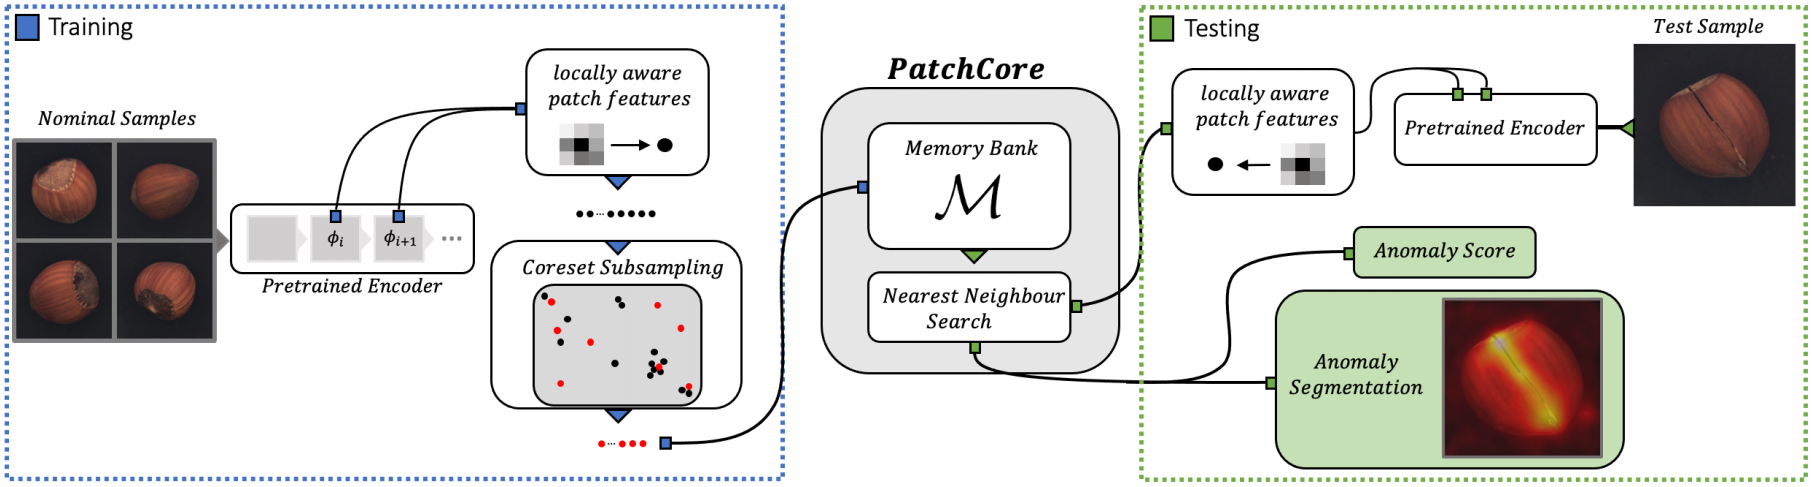
\includegraphics[width=1\linewidth]{images/architecture.png}
    \caption{PatchCore Architecture}
    \label{fig:architecture}
\end{figure}
\end{frame}

\begin{frame}{Training Phase}
\begin{block}{}
\begin{itemize}
    \item Input: Nominal or normal samples.
    \item Pretrained Encoder: 
    \begin{itemize}
        \item Extracts patch-level features ($\phi_i$).
        \item Uses WideResNet50-2 (a wider variant of ResNet-50 architecture) in the original PatchCore
    \end{itemize}
    \item Coreset Subsampling:
    \begin{itemize}
        \item Reduces feature set and stores representative embeddings in Memory Bank ($\mathcal{M}$).
    \end{itemize}
\end{itemize}
\end{block}
\begin{figure}
    \centering
    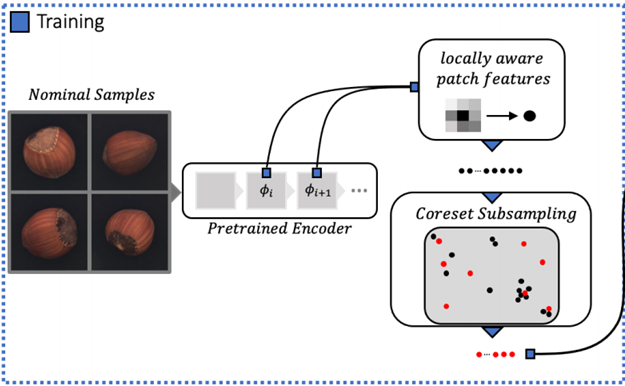
\includegraphics[width=0.4\linewidth]{images/training.png}
    \label{fig:training}
\end{figure}
\end{frame}

\begin{frame}{PatchCore Core Module}
\begin{block}{}
\begin{itemize}
    \item Memory bank ($\mathcal{M}$) holds selected features from nominal (normal) images
    \item During inference, features from test images will be compared to this memory bank.
\end{itemize}
\end{block}
\begin{figure}
    \centering
    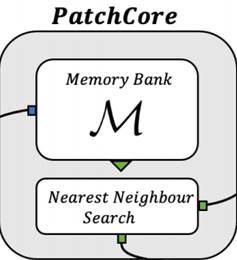
\includegraphics[width=0.3\linewidth]{images/core.png}
\end{figure}
\end{frame}

\begin{frame}{PatchCore Core Module}
\begin{block}{}
Finally, for all nominal training samples \( x_i \in \mathcal{X}_N \), the \textit{PatchCore} memory bank \( \mathcal{M} \) is then simply defined as
    \begin{equation}
    \mathcal{M} = \bigcup_{x_i \in \mathcal{X}_N} \mathcal{P}_{s,p} \left( \phi_j(x_i) \right).
    \end{equation}
    \noindent
    \textbf{Where:}
    \begin{itemize}
        \item \( \mathcal{X}_N \): Set of all nominal (normal) training samples.
        \item \( x_i \in \mathcal{X}_N \): A single image sample from the nominal dataset.
        \item \( \phi_j(x_i) \): Feature embedding of image \(x_i\) obtained from the \(j\)-th layer of a pretrained backbone network (WideResNet-50-2 or Vision Transformer for example).
        \item \( \mathcal{P}_{s,p}(\cdot) \): A patch sampling function that extracts a set of patch-level features from the embedding, using spatial stride \(s\) and patch size or proportion \(p\).
        \item \( \mathcal{M} \): The final memory bank, a collection of representative patch-level embeddings used during anomaly detection.
    \end{itemize}
\end{block}
\end{frame}

\begin{frame}{Testing Phase}
\begin{block}{}
\begin{itemize}
    \item \textbf{Input:} New (possibly anomalous) sample.
    \item Extract patch features using the same pretrained encoder.
    \item For each patch, find the nearest neighbor in $\mathcal{M}$.
    \item Compute:
    \begin{itemize}
        \item \textbf{Anomaly Score:} Based on distance.
        \item \textbf{Anomaly Segmentation:} Heatmap showing anomalous regions.
    \end{itemize}
\end{itemize}
\end{block}
\begin{figure}
    \centering
    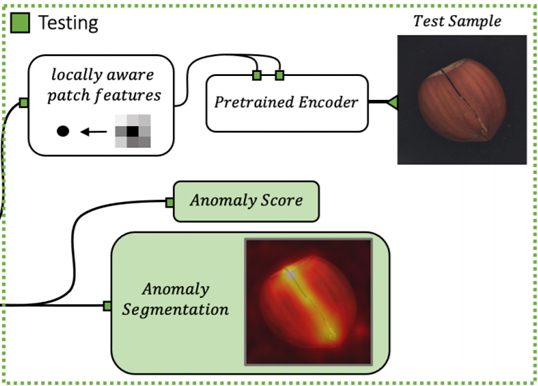
\includegraphics[width=0.35\linewidth]{images/testing.png}
\end{figure}
\end{frame}

